\section{Experimental Results}
\noindent \textbf{Amplification}\\
As mentioned before, the term "DNS reflection and amplification attack" derives from the two key elements involved in the attack methodology. In particular, to achieve amplification the attacker queries the DNS server, which will reply with larger responses than the original requests. In our project, we conducted various tests to explore different amplification factors based on the DNS request used.\\
We have compiled a summary table showcasing the types of DNS requests used, the corresponding response dimensions, and the amplification factors achieved. The table, shown below, provides a comprehensive overview of these metrics.
\begin{table}[H]
    \centering
    \resizebox{\columnwidth}{!}{%
        \begin{tabular}{|l|c|c|c|c|c|}
            \hline
            \textbf{Type} & \textbf{Request} & \textbf{A} & \textbf{MX} & \textbf{NS} & \textbf{ANY} \\
            \hline
            \textbf{Dimension (bytes)} & 74 & 108 & 306 & 330 & 540 \\
            \hline 
            \begin{tabular}[c]{@{}c@{}}\textbf{Amplification} \\ \textbf{Factor}\end{tabular} & - & 1.46 & 4.14 & 4.46 & 7.30 \\
            \hline 
        \end{tabular}%
    }
    \label{tab:dns-amplification}
\end{table}
\noindent \textbf{Effects on the Target}\\
To assess the effects of the DNS reflection attack, various metrics of the targeted system were measured with regards to performance and network aspects. Regarding the network, the target was used as the primary vantage point, and latency was measured using the ping and dig command tools. The measurement process was divided into three sections to analyze the performance differences. Initially, measurements were taken for a minute without any attack. This established a baseline for normal system performance. Subsequently, a two-minute attack was executed, involving the transmission of 10,000 packets per second to the DNS server by multiple attackers. Finally, an additional minute of measurements without any attack was conducted to detect any potential lingering disturbance effects.\\
The latency graph related to DNS queries presented in Figure \ref{fig:Query_MA_ANY1} visually demonstrates the impact of the attack over time. To improve visualization, a moving average of the latency time was applied, revealing a clear trend of increased latency during the attack. This trick becomes particularly helpful considering the inherent instability of latency measurements.
\begin{figure}[H]
    \centering
    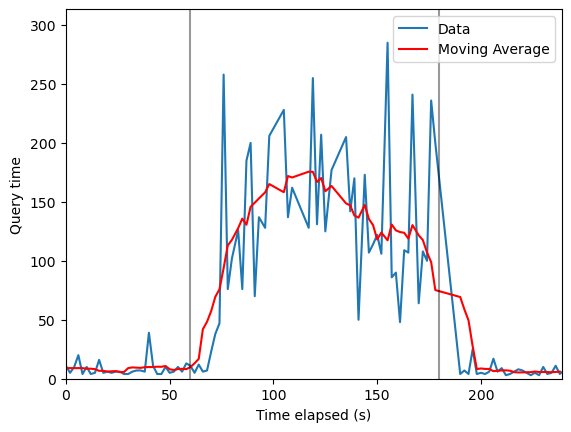
\includegraphics[width=\columnwidth]{Sections/Images/Query_MA_ANY.png}
    \caption{Evolution of the query time over the course of the test with the records of type ANY. The moving average better shows how the latency changes.}
    \label{fig:Query_MA_ANY1}
\end{figure}

\noindent \textbf{Server Performance}\\
Based on the type, victim and server have different performances.\\
%\begin{figure}[H]
%    \centering
%    
\includegraphics[width=\columnwidth]{Sections/Images/example.png}
%   \caption{Example image on one column}
%    \label{fig:example}
%\end{figure}
\noindent Text after the image.\\
{\bfseries DNS latency of the victim}\\
{\bfseries Ping latency of the victim}\\